\section{\ac{SAT}-солверы}

Сравнивать SMT с SAT, это как сравнивать высокоуровневый ЯП с языком ассемблера.
Последний может быть куда более эффективным, но на нем труднее программировать.

\subsection{CNF форма}

\ac{CNF}\footnote{\url{https://en.wikipedia.org/wiki/Conjunctive_normal_form}} это так называемая \textit{нормальная форма}.

% TODO recheck
% TODO write abt it!
%\textit{normal form} is somewhat similar to polynomials in algebra. 
%What is polynomial?
%It is a standard way to express unsystematic equations like $2x \cdot x$ as $3x$ polynomial, 
%and so you will be able to apply some operations to polynomials like summing, etc.

Любое булево выражение может быть сконвертировано в \textit{нормальную форму}, и \ac{CNF} это одна из них.
\ac{CNF}-выражение это пачка клозов (подвыражений) состоящих их литералов (или термов, переменных), операций ИЛИ и НЕ,
все из которых склеены друг с другом в полное выражение операцией И.
Вот способ запомнить: \ac{CNF} это ``И всех ИЛИ'' (или ``произведение всех сумм'')
и \ac{DNF} это ``ИЛИ всех И'' (или ``сумма всех произведений'').

Пример: $(\neg A \vee B) \wedge (C \vee \neg D)$.

$\vee$ означает ИЛИ (логическая дизьюнкция\footnote{\url{https://en.wikipedia.org/wiki/Logical_disjunction}}), 
знак ``+'' также иногда используется для ИЛИ.

$\wedge$ означает ИЛИ (логическая коньюнкция\footnote{\url{https://en.wikipedia.org/wiki/Logical_conjunction}}).
Легко запомнить: $\wedge$ выглядит как буква ``A''.
Знак ``$\cdot$'' также иногда используется для И.

$\neg$ это отрицание (НЕ).

% TODO A/B is the first clause, C/D is second

\subsection{Пример: двухбитный сумматор}
\label{adder}

В сущности, \ac{SAT}-солвер это солвер огромных булевых уравнений в CNF-форме.
Он просто выдает ответ, есть ли набор входных значений, удовлетворяющий CNF-выражению, и какие это значения должны быть.

Вот для примера двухбитный сумматор:

\begin{figure}[ht!]
\centering
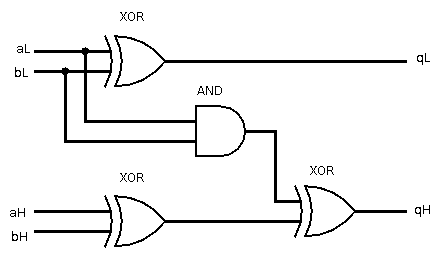
\includegraphics[scale=0.75]{SAT/adder_logisim.png}
\caption{Схема двухбитного сумматора}
\end{figure}

Сумматор здесь в самом простом возможном виде: у него нет входных и выходных переносов, и тут только 3 XOR-гейта
и один AND-гейт.
Попробуем разобраться, какой набор входных переменных заставит сумматор выставить оба выходных бита?
Просто подсчитав в уме, мы можем увидеть, что таких способа 4: $0+3=3$, $1+2=3$, $2+1=3$, $3+0=3$.
Вот также таблица истинности, с подсвеченными соответствующими рядами:

\newcommand{\HLcell}{\cellcolor{blue!25}}

\begin{center}
\begin{doublespace}
\noindent\(\begin{array}{l|llllll}
  & \text{aH} & \text{aL} & \text{bH} & \text{bL} & \text{qH} & \text{qL} \\
\hline
 \text{3+3 = 6 $\equiv $ 2 (mod 4)} & 1 & 1 & 1 & 1 & 1 & 0 \\
 \text{3+2 = 5 $\equiv $ 1 (mod 4)} & 1 & 1 & 1 & 0 & 0 & 1 \\
 \text{3+1 = 4 $\equiv $ 0 (mod 4)} & 1 & 1 & 0 & 1 & 0 & 0 \\
 \text{\HLcell{}3+0 = 3 $\equiv $ 3 (mod 4)} & \HLcell{}1 & \HLcell{}1 & \HLcell{}0 & \HLcell{}0 & \HLcell{}1 & \HLcell{}1 \\
 \text{2+3 = 5 $\equiv $ 1 (mod 4)} & 1 & 0 & 1 & 1 & 0 & 1 \\
 \text{2+2 = 4 $\equiv $ 0 (mod 4)} & 1 & 0 & 1 & 0 & 0 & 0 \\
 \text{\HLcell{}2+1 = 3 $\equiv $ 3 (mod 4)} & \HLcell{}1 & \HLcell{}0 & \HLcell{}0 & \HLcell{}1 & \HLcell{}1 & \HLcell{}1 \\
 \text{2+0 = 2 $\equiv $ 2 (mod 4)} & 1 & 0 & 0 & 0 & 1 & 0 \\
 \text{1+3 = 4 $\equiv $ 0 (mod 4)} & 0 & 1 & 1 & 1 & 0 & 0 \\
 \text{\HLcell{}1+2 = 3 $\equiv $ 3 (mod 4)} & \HLcell{}0 & \HLcell{}1 & \HLcell{}1 & \HLcell{}0 & \HLcell{}1 & \HLcell{}1 \\
 \text{1+1 = 2 $\equiv $ 2 (mod 4)} & 0 & 1 & 0 & 1 & 1 & 0 \\
 \text{1+0 = 1 $\equiv $ 1 (mod 4)} & 0 & 1 & 0 & 0 & 0 & 1 \\
 \text{\HLcell{}0+3 = 3 $\equiv $ 3 (mod 4)} & \HLcell{}0 & \HLcell{}0 & \HLcell{}1 & \HLcell{}1 & \HLcell{}1 & \HLcell{}1 \\
 \text{0+2 = 2 $\equiv $ 2 (mod 4)} & 0 & 0 & 1 & 0 & 1 & 0 \\
 \text{0+1 = 1 $\equiv $ 1 (mod 4)} & 0 & 0 & 0 & 1 & 0 & 1 \\
 \text{0+0 = 0 $\equiv $ 0 (mod 4)} & 0 & 0 & 0 & 0 & 0 & 0 \\
\end{array}\)
\end{doublespace}
\end{center}


Посмотрим, что об этом скажет SAT-солвер?

В начале, нам нужно представить наш двухбитный сумматор как CNF-выражение.

Используя Wolfram Mathematica, можно выразить 1-битное выражение для обоих выходов сумматоров:\\
\\
\textbf{\texttt{In[]:=AdderQ0[aL$\_$,bL$\_$]=Xor[aL,bL]}} \\
\textbf{\texttt{Out[]:=aL $\veebar$ bL}} \\
\\
\textbf{\texttt{In[]:=AdderQ1[aL$\_$,aH$\_$,bL$\_$,bH$\_$]=Xor[And[aL,bL],Xor[aH,bH]]}} \\
\textbf{\texttt{Out[]:=aH $\veebar$ bH $\veebar$ (aL \&\& bL)}} \\
\\
Нам нужно такое выражение, где обе части выдадут единицы.
Используя Wolfram Mathematica, найдем все возможные входы такого выражения (я склеил обе части при помощи And): \\
\\
\textbf{\texttt{In[]:=Boole[SatisfiabilityInstances[And[AdderQ0[aL,bL],AdderQ1[aL,aH,bL,bH]],\{aL,aH,bL,bH\},4]]}} \\
\textbf{\texttt{Out[]:=\{1,1,0,0\},\{1,0,0,1\},\{0,1,1,0\},\{0,0,1,1\}}} \\
\\
Да, действительно, Mathematica говорит, что здесь 4 входа, которые приведут к нужному нам результату.
Так что, Mathematica тоже может использоваться как \ac{SAT}-солвер.

Тем не менее, перейдем к CNF-форме. Используя Mathematica, сконвертируем наше выражение в CNF-форму:\\
\\
\textbf{\texttt{In[]:=cnf=BooleanConvert[And[AdderQ0[aL,bL],AdderQ1[aL,aH,bL,bH]],``CNF'']}} \\
\textbf{\texttt{Out[]:=(!aH $\|$ !bH) \&\& (aH $\|$ bH) \&\& (!aL $\|$ !bL) \&\& (aL $\|$ bL)}} \\
\\
Выглядит посложнее. Причина такой многословности в том, что \ac{CNF}-форма не поддерживает операцию исключающего
ИЛИ.
% FIXME: TeX form of the expression!

\subsubsection{MiniSat}

Для начала, попробуем MiniSat\footnote{\url{http://minisat.se/MiniSat.html}}.
Стандартный способ закодировать \ac{CNF}-выражение для MiniSat это перечислить все части ИЛИ в каждой строке.
Также, MiniSat не поддерживает имена переменных, только числа.
Перечислим наши переменные: 1 будет aH, 2 -- aL, 3 -- bH, 4 -- bL.

Вот что получилось, когда я сконвертировал выражение из Mathematica во входной файл для MiniSat:

\begin{lstlisting}
p cnf 4 4
-1 -3 0
1 3 0
-2 -4 0
2 4 0
\end{lstlisting}

Две четверки в первой строке это, соответственно, число переменных и число клозов.
Так что тут 4 строки, каждая для каждого клоза ИЛИ.
Минус перед номером переменной означает что переменная инвертирована.
Отсутствие минуса -- не инвертирована.
Ноль в конце это просто оконечивающий ноль, означающий конец клоза.

Другими словами, каждая строка это ИЛИ-клоз с возможными инвертированиями,
и задача MiniSat в том, чтобы найти такой набор входных переменных, который удовлетворит все строки во входном файле.

Этот файл я назвал \textit{adder.cnf} и теперь попробуем MiniSat:

\begin{lstlisting}
% minisat -verb=0 adder.cnf results.txt
SATISFIABLE
\end{lstlisting}

Результаты в файле \textit{results.txt}:

\begin{lstlisting}
SAT
-1 -2 3 4 0
\end{lstlisting}

Это означает, что если первые две переменных (aH и aL) будут \textit{false},
и две последние переменные (bH и bL) будут \textit{true},
все \ac{CNF}-выражение будет истинно (satisfiable).
Похоже на правду: если bH и bL выставить в \textit{true}, оба бита результата также будут \textit{true}.

Как получить другие решения (instances)?
\ac{SAT}-солверы, как и \ac{SMT}-солверы, выдают только одно решение (или \textit{instance}).

MiniSat использует \ac{PRNG}, и его изначальное состояние (seed) можно задать явно.
Я попробовал разные значения, но результат всё тот же.
Тем не менее, CryptoMiniSat в этом случае может показать все возможные 4 решения, хотя и в хаотичном порядке.
Так что это не очень надежный способ.

Видимо, единственный способ, это инвертировать клоз решения и добавить его во входное выражение.
Мы получили \TT{-1 -2 3 4}, 
теперь мы можем инвертировать все значения в нем (просто поменяйте минусы: \TT{1 2 -3 -4}),
и добавим это в конец входного файла:

\begin{lstlisting}
p cnf 4 5
-1 -3 0
1 3 0
-2 -4 0
2 4 0
1 2 -3 -4
\end{lstlisting}

Получаем другой результат:

\begin{lstlisting}
SAT
1 2 -3 -4 0
\end{lstlisting}

Это означает что обе aH и aL должны быть \textit{true} и bH и bL должны быть \textit{false}, чтобы удовлетворить
входное выражение.
Снова инвертируем это решение и снова добавим:

\begin{lstlisting}
p cnf 4 6
-1 -3 0
1 3 0
-2 -4 0
2 4 0
1 2 -3 -4
-1 -2 3 4 0
\end{lstlisting}

Результат:

\begin{lstlisting}
SAT
-1 2 3 -4 0
\end{lstlisting}

aH=false, aL=true, bH=true, bL=false. Это также корректно, в соответствии с таблицей истинности.

Добавим снова:

\begin{lstlisting}
p cnf 4 7
-1 -3 0
1 3 0
-2 -4 0
2 4 0
1 2 -3 -4
-1 -2 3 4 0
1 -2 -3 4 0
\end{lstlisting}

\begin{lstlisting}
SAT
1 -2 -3 4 0
\end{lstlisting}

\textit{aH=true, aL=false, bH=false, bL=true.} Это тоже верно.

Это четвертый результат. Больше быть не должно. Что если добавим и это?

\begin{lstlisting}
p cnf 4 8
-1 -3 0
1 3 0
-2 -4 0
2 4 0
1 2 -3 -4
-1 -2 3 4 0
1 -2 -3 4 0
-1 2 3 -4 0
\end{lstlisting}

Теперь MiniSat просто говорит ``UNSATISFIABLE'' без всякой дополнительной информации в файле результатов.

Нам пример крохотный, но MiniSat может работать с огромными \ac{CNF}-выражениями.

\subsubsection{CryptoMiniSat}

Операция исключающего ИЛИ (XOR) отсутствует в CNF-форме, но она очень важна в криптографических алгоритмах.
Простейший способ представить одну единственную XOR-операцию в CNF-форме, это:
$(\neg x \vee \neg y) \wedge (x \vee y)$ -- не очень короткое выражение,
хотя, множество XOR-операций в одном выражении могут оптимизироваться лучше.

Одна значительная разница между MiniSat и CryptoMiniSat в том, что последний поддерживает
клозы с операцией XOR вместо ИЛИ,
потому что CryptoMiniSat предназначен больше для анализа криптоалгоритмов\footnote{\url{http://www.msoos.org/xor-clauses/}}.
XOR-клозы поддерживаются в CryptoMiniSat специальным образом, без трансляции в клозы ИЛИ.

Вам нужно просто прибавить ``x'' к клозу в \ac{CNF}-файле и CryptoMiniSat затем считает обычный ИЛИ-клоз как XOR-клоз.
Что до двухбитного сумматора, вот самое короткое из возможных XOR-CNF выражений, которое можно использовать
для поиска всех входных значений, где оба выходных бита выставлены:

$(aH \oplus bH) \wedge (aL \oplus bL)$

Это \TT{.cnf}-файл CryptoMiniSat:

\begin{lstlisting}
p cnf 4 2
x1 3 0
x2 4 0
\end{lstlisting}

Запускаю CryptoMiniSat с разными значениями для инициализации его \ac{PRNG} \dots

\begin{lstlisting}
% cryptominisat4 --verb 0 --random 0 XOR_adder.cnf
s SATISFIABLE
v 1 2 -3 -4 0
% cryptominisat4 --verb 0 --random 1 XOR_adder.cnf
s SATISFIABLE
v -1 -2 3 4 0
% cryptominisat4 --verb 0 --random 2 XOR_adder.cnf
s SATISFIABLE
v 1 -2 -3 4 0
% cryptominisat4 --verb 0 --random 3 XOR_adder.cnf
s SATISFIABLE
v 1 2 -3 -4 0
% cryptominisat4 --verb 0 --random 4 XOR_adder.cnf
s SATISFIABLE
v -1 2 3 -4 0
% cryptominisat4 --verb 0 --random 5 XOR_adder.cnf
s SATISFIABLE
v -1 2 3 -4 0
% cryptominisat4 --verb 0 --random 6 XOR_adder.cnf
s SATISFIABLE
v -1 -2 3 4 0
% cryptominisat4 --verb 0 --random 7 XOR_adder.cnf
s SATISFIABLE
v 1 -2 -3 4 0
% cryptominisat4 --verb 0 --random 8 XOR_adder.cnf
s SATISFIABLE
v 1 2 -3 -4 0
% cryptominisat4 --verb 0 --random 9 XOR_adder.cnf
s SATISFIABLE
v 1 2 -3 -4 0
\end{lstlisting}

Тем не менее, все 4 возможных решения, это:

\begin{lstlisting}
v -1 -2 3 4 0
v -1 2 3 -4 0
v 1 -2 -3 4 0
v 1 2 -3 -4 0
\end{lstlisting}

\dots то же, что и выдал MiniSat.

% subsections:
\subsection{Cracking Minesweeper with SAT solver}
\label{minesweeper_SAT}

See also about cracking it using Z3: \ref{minesweeper_SMT}.

SAT solvers are very different in that sense that they are at low-level, and can take only CNF expressions on input.

\subsubsection{Simple population count function}

First of all, somehow we need to count neighbour bombs.
The counting function is very similar to \textit{population count} function.

We can try to make CNF expression in Wolfram Mathematica.
This will be a function, returning True if any of 2 bits of 8 inputs bits are True and others are False.
First, we make truth table of such function:

\begin{lstlisting}
In[]:= tbl2 = 
 Table[PadLeft[IntegerDigits[i, 2], 8] -> 
   If[Equal[DigitCount[i, 2][[1]], 2], 1, 0], {i, 0, 255}]

Out[]= {{0, 0, 0, 0, 0, 0, 0, 0} -> 0, {0, 0, 0, 0, 0, 0, 0, 1} -> 0, 
{0, 0, 0, 0, 0, 0, 1, 0} -> 0, {0, 0, 0, 0, 0, 0, 1, 1} -> 1, 
{0, 0, 0, 0, 0, 1, 0, 0} -> 0, {0, 0, 0, 0, 0, 1, 0, 1} -> 1, 
{0, 0, 0, 0, 0, 1, 1, 0} -> 1, {0, 0, 0, 0, 0, 1, 1, 1} -> 0, 
{0, 0, 0, 0, 1, 0, 0, 0} -> 0, {0, 0, 0, 0, 1, 0, 0, 1} -> 1, 
{0, 0, 0, 0, 1, 0, 1, 0} -> 1, {0, 0, 0, 0, 1, 0, 1, 1} -> 0, 
...
{1, 1, 1, 1, 1, 0, 1, 0} -> 0, {1, 1, 1, 1, 1, 0, 1, 1} -> 0, 
{1, 1, 1, 1, 1, 1, 0, 0} -> 0, {1, 1, 1, 1, 1, 1, 0, 1} -> 0, 
{1, 1, 1, 1, 1, 1, 1, 0} -> 0, {1, 1, 1, 1, 1, 1, 1, 1} -> 0}
\end{lstlisting}

Now we can make CNF expression using this truth table:

\begin{lstlisting}
In[]:= BooleanConvert[
 BooleanFunction[tbl2, {a, b, c, d, e, f, g, h}], "CNF"]

Out[]= (! a || ! b || ! c) && (! a || ! b || ! d) && (! a || ! 
    b || ! e) && (! a || ! b || ! f) && (! a || ! b || ! g) && (! 
    a || ! b || ! h) && (! a || ! c || ! d) && (! a || ! c || ! 
    e) && (! a || ! c || ! f) && (! a || ! c || ! g) && (! a || ! 
    c || ! h) && (! a || ! d || ! e) && (! a || ! d || ! f) && (! 
    a || ! d || ! g) && (! a || ! d || ! h) && (! a || ! e || ! 
    f) && (! a || ! e || ! g) && (! a || ! e || ! h) && (! a || ! 
    f || ! g) && (! a || ! f || ! h) && (! a || ! g || ! h) && (a || 
   b || c || d || e || f || g) && (a || b || c || d || e || f || 
   h) && (a || b || c || d || e || g || h) && (a || b || c || d || f ||
    g || h) && (a || b || c || e || f || g || h) && (a || b || d || 
   e || f || g || h) && (a || c || d || e || f || g || 
   h) && (! b || ! c || ! d) && (! b || ! c || ! e) && (! b || ! 
    c || ! f) && (! b || ! c || ! g) && (! b || ! c || ! h) && (! 
    b || ! d || ! e) && (! b || ! d || ! f) && (! b || ! d || ! 
    g) && (! b || ! d || ! h) && (! b || ! e || ! f) && (! b || ! 
    e || ! g) && (! b || ! e || ! h) && (! b || ! f || ! g) && (! 
    b || ! f || ! h) && (! b || ! g || ! h) && (b || c || d || e || 
   f || g || 
   h) && (! c || ! d || ! e) && (! c || ! d || ! f) && (! c || ! 
    d || ! g) && (! c || ! d || ! h) && (! c || ! e || ! f) && (! 
    c || ! e || ! g) && (! c || ! e || ! h) && (! c || ! f || ! 
    g) && (! c || ! f || ! h) && (! c || ! g || ! h) && (! d || ! 
    e || ! f) && (! d || ! e || ! g) && (! d || ! e || ! h) && (! 
    d || ! f || ! g) && (! d || ! f || ! h) && (! d || ! g || ! 
    h) && (! e || ! f || ! g) && (! e || ! f || ! h) && (! e || ! 
    g || ! h) && (! f || ! g || ! h)
\end{lstlisting}

The syntax is similar to C/C++.
Let's check it.

I wrote a Python function to convert Mathematica's output into CNF file which can be feeded to SAT solver:

\lstinputlisting{SAT/minesweeper/tst.py}

It replaces a/b/c/... variables to the variable names passed (1/2/3...), reworks syntax, etc.
Here is a result:

\lstinputlisting{SAT/minesweeper/tst1.cnf}

I can run it:

\begin{lstlisting}
% minisat -verb=0 tst1.cnf results.txt
WARNING: for repeatability, setting FPU to use double precision
SATISFIABLE

% cat results.txt
SAT
1 -2 -3 -4 -5 -6 -7 8 0
\end{lstlisting}

The variable name in results lacking minus sign is "True".
Variable name with minus sign is "False".
We see there are just two variables are "True": 1 and 8.
This is indeed correct: MiniSat solver found a condition, for which our function returns "True".
Zero at the end is just a terminal symbol which means nothing.

We can ask MiniSat for another solution, by adding current solution to the input CNF file, but with all variables negated:

\begin{lstlisting}
...
-5 -6 -8 0
-5 -7 -8 0
-6 -7 -8 0
-1 2 3 4 5 6 7 -8 0
\end{lstlisting}

In plain English language, this means "give me ANY solution which can satisfy all clauses, but also not equal to the last clause we've just added".

MiniSat, indeed, found another solution, again, with only 2 variables equal to "True":

\begin{lstlisting}
% minisat -verb=0 tst2.cnf results.txt
WARNING: for repeatability, setting FPU to use double precision
SATISFIABLE

% cat results.txt
SAT
1 2 -3 -4 -5 -6 -7 -8 0
\end{lstlisting}

By the way, <i>population count</i> function for 8 neighbours in CNF form is simplest:

\begin{lstlisting}
a&&b&&c&&d&&e&&f&&g&&h
\end{lstlisting}

Indeed: it's true if all 8 input bits are "True".

The function for 0 neighbours is also simple:

\begin{lstlisting}
!a&&!b&&!c&&!d&&!e&&!f&&!g&&!h
\end{lstlisting}

It means, it will return "True", if all input variables are "False".

By the way, function for POPCNT1 is also simple:

\begin{lstlisting}
(!a||!b)&&(!a||!c)&&(!a||!d)&&(!a||!e)&&(!a||!f)&&(!a||!g)&&(!a||!h)&&(a||b||c||d||e||f||g||h)&&
(!b||!c)&&(!b||!d)&&(!b||!e)&&(!b||!f)&&(!b||!g)&&(!b||!h)&&(!c||!d)&&(!c||!e)&&(!c||!f)&&(!c||!g)&&
(!c||!h)&&(!d||!e)&&(!d||!f)&&(!d||!g)&&(!d||!h)&&(!e||!f)&&(!e||!g)&&(!e||!h)&&(!f||!g)&&(!f||!h)&&(!g||!h)
\end{lstlisting}

It just enumerates all possible pairs of 8 variables (a/b, a/c, a/d, etc) and says: no two bits must be present
simultaneously in each possible pair.
And there is another clause: "(a||b||c||d||e||f||g||h)", which says: at least one bit must be present among 8 variables.

And yes, you can ask Mathematica for finding CNF expressions for any other truth table.

\subsubsection{Minesweeper}

Now we can use Mathematica to get all \textit{population count} functions for 0..8 neighbours.

For 9*9 Minesweeper grid including invisible border, there will be 11*11=121 variables, mapped to Minesweeper grid like this:

\begin{lstlisting}
 1    2   3   4   5   6   7   8   9  10  11
12   13  14  15  16  17  18  19  20  21  22
23   24  25  26  27  28  29  30  31  32  33
34   35  36  37  38  39  40  41  42  43  44

...

100 101 102 103 104 105 106 107 108 109 110
111 112 113 114 115 116 117 118 119 120 121
\end{lstlisting}

Then we write a Python script which stacks all \textit{population count} functions: each function for each known number of neighbours (digit on Minesweeper field).
Each POPCNTx() function takes list of variable numbers and outputs list of clauses to be added to the final CNF file.

As of empty cells, we also add them as clauses, but with minus sign, which means, the variable must be False.
Whenever we try to place bomb, we add its variable as clause without minus sign, this means the variable must be True.

Then we execute external minisat process.
The only thing we need from it is exit code.
If an input CNF is UNSAT, it returns 20:

\lstinputlisting{SAT/minesweeper/minesweeper_SAT.py}

The output CNF file can be large, up to ~2000 clauses, or more, here is an example: \url{https://github.com/dennis714/SAT_SMT_article/blob/master/SAT/minesweeper/sample.cnf}.

Anyway, it works just like my previous Z3Py script:

\begin{lstlisting}
row=1, col=3, unsat!
row=6, col=2, unsat!
row=6, col=3, unsat!
row=7, col=4, unsat!
row=7, col=9, unsat!
row=8, col=9, unsat!
\end{lstlisting}

... but it runs way faster, even considering overhead of executing external program.
Perhaps, Z3Py version could be optimized much better?

The files, including Wolfram Mathematica notebook: \url{https://github.com/dennis714/SAT_SMT_article/tree/master/SAT/minesweeper}.


\subsection{Conway's Game of Life and SAT solver}

\subsubsection{Part I: reversing back state of ``Game of Life''}

How could we reverse back a known state of GoL?
This can be solved by brute-force, but this is extremely slow and inefficient.

Let's try to use SAT solver.

First, we need to define a function which will tell, if the new cell will be created/born, preserved/stay or died.
Quick refresher: cell is born if it has 3 neighbours, it stays alive if it has 2 or 3 neighbours, it dies in any other case.

This is how I can define a function reflecting state of a new cell in the next state:

\begin{lstlisting}
if center==true:
	return popcnt2(neighbours) || popcnt3(neighbours)
if center==false
	return popcnt3(neighbours)
\end{lstlisting}

We can get rid of ``if'' construction:

\begin{lstlisting}
result=(center=true && (popcnt2(neighbours) || popcnt3(neighbours))) || (center=false && popcnt3(neighbours))
\end{lstlisting}

... where ``center'' is state of central cell, ``neighbours'' are 8 neighbouring cells, popcnt2 is a function which
returns True if it has exactly 2 bits on input, popcnt3 is the same, but for 3 bits
(just like these were used in my "Minesweeper" example (\ref{minesweeper_SAT}).

Using Wolfram Mathematica, I first create all helper functions and truth table for the function, which returns "true",
if a cell must be present in the next state, or "false" if not:

\begin{lstlisting}
In[1]:= popcount[n_Integer]:=IntegerDigits[n,2] // Total

In[2]:= popcount2[n_Integer]:=Equal[popcount[n],2]

In[3]:= popcount3[n_Integer]:=Equal[popcount[n],3]

In[4]:= newcell[center_Integer,neighbours_Integer]:=(center==1 && (popcount2[neighbours]|| popcount3[neighbours]))||
(center==0 && popcount3[neighbours])

In[13]:= NewCellIsTrue=Flatten[Table[Join[{center},PadLeft[IntegerDigits[neighbours,2],8]] ->
Boole[newcell[center, neighbours]],{neighbours,0,255},{center,0,1}]]

Out[13]= {{0,0,0,0,0,0,0,0,0}->0,
{1,0,0,0,0,0,0,0,0}->0,
{0,0,0,0,0,0,0,0,1}->0,
{1,0,0,0,0,0,0,0,1}->0,
{0,0,0,0,0,0,0,1,0}->0,
{1,0,0,0,0,0,0,1,0}->0,
{0,0,0,0,0,0,0,1,1}->0,
{1,0,0,0,0,0,0,1,1}->1,

...

\end{lstlisting}

Now we can create a CNF expression out of truth table:

\begin{lstlisting}
In[14]:= BooleanConvert[BooleanFunction[NewCellIsTrue,{center,a,b,c,d,e,f,g,h}],"CNF"]
Out[14]= (!a||!b||!c||!d)&&(!a||!b||!c||!e)&&(!a||!b||!c||!f)&&(!a||!b||!c||!g)&&(!a||!b||!c||!h)&&(!a||!b||!d||!e)&&
(!a||!b||!d||!f)&&(!a||!b||!d||!g)&&(!a||!b||!d||!h)&&(!a||!b||!e||!f)&&(!a||!b||!e||!g)&&(!a||!b||!e||!h)&&
(!a||!b||!f||!g)&&(!a||!b||!f||!h)&&(!a||!b||!g||!h)&&(!a||!c||!d||!e)&&(!a||!c||!d||!f)&&(!a||!c||!d||!g)&&
(!a||!c||!d||!h)&&(!a||!c||!e||!f)&&(!a||!c||!e||!g)&&(!a||!c||!e||!h)&&(!a||!c||!f||!g)&&(!a||!c||!f||!h)&&

...

\end{lstlisting}

Also, we need a second function, "inverted" one, which will return "true" if the cell must be absent in the next state,
or "false" otherwise:

\begin{lstlisting}
In[15]:= NewCellIsFalse=Flatten[Table[Join[{center},PadLeft[IntegerDigits[neighbours,2],8]] ->
Boole[Not[newcell[center, neighbours]]],{neighbours,0,255},{center,0,1}]]
Out[15]= {{0,0,0,0,0,0,0,0,0}->1,
{1,0,0,0,0,0,0,0,0}->1,
{0,0,0,0,0,0,0,0,1}->1,
{1,0,0,0,0,0,0,0,1}->1,
{0,0,0,0,0,0,0,1,0}->1,

...

In[16]:= BooleanConvert[BooleanFunction[NewCellIsFalse,{center,a,b,c,d,e,f,g,h}],"CNF"]
Out[16]= (!a||!b||!c||d||e||f||g||h)&&(!a||!b||c||!d||e||f||g||h)&&(!a||!b||c||d||!e||f||g||h)&&
(!a||!b||c||d||e||!f||g||h)&&(!a||!b||c||d||e||f||!g||h)&&(!a||!b||c||d||e||f||g||!h)&&
(!a||!b||!center||d||e||f||g||h)&&(!a||b||!c||!d||e||f||g||h)&&(!a||b||!c||d||!e||f||g||h)&&
(!a||b||!c||d||e||!f||g||h)&&(!a||b||!c||d||e||f||!g||h)&&(!a||b||!c||d||e||f||g||!h)&&
(!a||b||c||!d||!e||f||g||h)&&(!a||b||c||!d||e||!f||g||h)&&(!a||b||c||!d||e||f||!g||h)&&

...

\end{lstlisting}

Using the very same way as in my "Minesweeper" example, I can convert CNF expression to list of clauses:

\begin{lstlisting}
def mathematica_to_CNF (s, center, a):
    s=s.replace("center", center)
    s=s.replace("a", a[0]).replace("b", a[1]).replace("c", a[2]).replace("d", a[3])
    s=s.replace("e", a[4]).replace("f", a[5]).replace("g", a[6]).replace("h", a[7])
    s=s.replace("!", "-").replace("||", " ").replace("(", "").replace(")", "")
    s=s.split ("&&")
    return s
\end{lstlisting}

And again, as in "Minesweeper", there is an invisible border, to make processing simpler.
SAT variables are also numbered as in previous example:

\begin{lstlisting}
 1    2   3   4   5   6   7   8   9  10  11
12   13  14  15  16  17  18  19  20  21  22
23   24  25  26  27  28  29  30  31  32  33
34   35  36  37  38  39  40  41  42  43  44

...

100 101 102 103 104 105 106 107 108 109 110
111 112 113 114 115 116 117 118 119 120 121
\end{lstlisting}

Also, there is a visible border, always fixed to "False", to make things simpler.

Now the working source code.
Whenever we encounter "*" in final\_state[], we add clauses generated by cell\_is\_true() function,
or cell\_is\_false() if otherwise.
When we get a solution, it is negated and added to the list of clauses, so when minisat is executed next time,
it will skip solution which was already printed.

\begin{lstlisting}
...

def cell_is_false (center, a):
    s="(!a||!b||!c||d||e||f||g||h)&&(!a||!b||c||!d||e||f||g||h)&&(!a||!b||c||d||!e||f||g||h)&&" \
      "(!a||!b||c||d||e||!f||g||h)&&(!a||!b||c||d||e||f||!g||h)&&(!a||!b||c||d||e||f||g||!h)&&" \
      "(!a||!b||!center||d||e||f||g||h)&&(!a||b||!c||!d||e||f||g||h)&&(!a||b||!c||d||!e||f||g||h)&&" \
      "(!a||b||!c||d||e||!f||g||h)&&(!a||b||!c||d||e||f||!g||h)&&(!a||b||!c||d||e||f||g||!h)&&" \
      "(!a||b||c||!d||!e||f||g||h)&&(!a||b||c||!d||e||!f||g||h)&&(!a||b||c||!d||e||f||!g||h)&&" \
      "(!a||b||c||!d||e||f||g||!h)&&(!a||b||c||d||!e||!f||g||h)&&(!a||b||c||d||!e||f||!g||h)&&" \
      "(!a||b||c||d||!e||f||g||!h)&&(!a||b||c||d||e||!f||!g||h)&&(!a||b||c||d||e||!f||g||!h)&&" \
      "(!a||b||c||d||e||f||!g||!h)&&(!a||!c||!center||d||e||f||g||h)&&(!a||c||!center||!d||e||f||g||h)&&" \
      "(!a||c||!center||d||!e||f||g||h)&&(!a||c||!center||d||e||!f||g||h)&&(!a||c||!center||d||e||f||!g||h)&&" \
      "(!a||c||!center||d||e||f||g||!h)&&(a||!b||!c||!d||e||f||g||h)&&(a||!b||!c||d||!e||f||g||h)&&" \
      "(a||!b||!c||d||e||!f||g||h)&&(a||!b||!c||d||e||f||!g||h)&&(a||!b||!c||d||e||f||g||!h)&&" \
      "(a||!b||c||!d||!e||f||g||h)&&(a||!b||c||!d||e||!f||g||h)&&(a||!b||c||!d||e||f||!g||h)&&" \
      "(a||!b||c||!d||e||f||g||!h)&&(a||!b||c||d||!e||!f||g||h)&&(a||!b||c||d||!e||f||!g||h)&&" \
      "(a||!b||c||d||!e||f||g||!h)&&(a||!b||c||d||e||!f||!g||h)&&(a||!b||c||d||e||!f||g||!h)&&" \
      "(a||!b||c||d||e||f||!g||!h)&&(a||b||!c||!d||!e||f||g||h)&&(a||b||!c||!d||e||!f||g||h)&&" \
      "(a||b||!c||!d||e||f||!g||h)&&(a||b||!c||!d||e||f||g||!h)&&(a||b||!c||d||!e||!f||g||h)&&" \
      "(a||b||!c||d||!e||f||!g||h)&&(a||b||!c||d||!e||f||g||!h)&&(a||b||!c||d||e||!f||!g||h)&&" \
      "(a||b||!c||d||e||!f||g||!h)&&(a||b||!c||d||e||f||!g||!h)&&(a||b||c||!d||!e||!f||g||h)&&" \
      "(a||b||c||!d||!e||f||!g||h)&&(a||b||c||!d||!e||f||g||!h)&&(a||b||c||!d||e||!f||!g||h)&&" \
      "(a||b||c||!d||e||!f||g||!h)&&(a||b||c||!d||e||f||!g||!h)&&(a||b||c||d||!e||!f||!g||h)&&" \
      "(a||b||c||d||!e||!f||g||!h)&&(a||b||c||d||!e||f||!g||!h)&&(a||b||c||d||e||!f||!g||!h)&&" \
      "(!b||!c||!center||d||e||f||g||h)&&(!b||c||!center||!d||e||f||g||h)&&(!b||c||!center||d||!e||f||g||h)&&" \
      "(!b||c||!center||d||e||!f||g||h)&&(!b||c||!center||d||e||f||!g||h)&&(!b||c||!center||d||e||f||g||!h)&&" \
      "(b||!c||!center||!d||e||f||g||h)&&(b||!c||!center||d||!e||f||g||h)&&(b||!c||!center||d||e||!f||g||h)&&" \
      "(b||!c||!center||d||e||f||!g||h)&&(b||!c||!center||d||e||f||g||!h)&&(b||c||!center||!d||!e||f||g||h)&&" \
      "(b||c||!center||!d||e||!f||g||h)&&(b||c||!center||!d||e||f||!g||h)&&(b||c||!center||!d||e||f||g||!h)&&" \
      "(b||c||!center||d||!e||!f||g||h)&&(b||c||!center||d||!e||f||!g||h)&&(b||c||!center||d||!e||f||g||!h)&&" \
      "(b||c||!center||d||e||!f||!g||h)&&(b||c||!center||d||e||!f||g||!h)&&(b||c||!center||d||e||f||!g||!h)"

    return mathematica_to_CNF(s, center, a)

def cell_is_true (center, a):
    s="(!a||!b||!c||!d)&&(!a||!b||!c||!e)&&(!a||!b||!c||!f)&&(!a||!b||!c||!g)&&(!a||!b||!c||!h)&&" \
      "(!a||!b||!d||!e)&&(!a||!b||!d||!f)&&(!a||!b||!d||!g)&&(!a||!b||!d||!h)&&(!a||!b||!e||!f)&&" \
      "(!a||!b||!e||!g)&&(!a||!b||!e||!h)&&(!a||!b||!f||!g)&&(!a||!b||!f||!h)&&(!a||!b||!g||!h)&&" \
      "(!a||!c||!d||!e)&&(!a||!c||!d||!f)&&(!a||!c||!d||!g)&&(!a||!c||!d||!h)&&(!a||!c||!e||!f)&&" \
      "(!a||!c||!e||!g)&&(!a||!c||!e||!h)&&(!a||!c||!f||!g)&&(!a||!c||!f||!h)&&(!a||!c||!g||!h)&&" \
      "(!a||!d||!e||!f)&&(!a||!d||!e||!g)&&(!a||!d||!e||!h)&&(!a||!d||!f||!g)&&(!a||!d||!f||!h)&&" \
      "(!a||!d||!g||!h)&&(!a||!e||!f||!g)&&(!a||!e||!f||!h)&&(!a||!e||!g||!h)&&(!a||!f||!g||!h)&&" \
      "(a||b||c||center||d||e||f)&&(a||b||c||center||d||e||g)&&(a||b||c||center||d||e||h)&&" \
      "(a||b||c||center||d||f||g)&&(a||b||c||center||d||f||h)&&(a||b||c||center||d||g||h)&&" \
      "(a||b||c||center||e||f||g)&&(a||b||c||center||e||f||h)&&(a||b||c||center||e||g||h)&&" \
      "(a||b||c||center||f||g||h)&&(a||b||c||d||e||f||g)&&(a||b||c||d||e||f||h)&&(a||b||c||d||e||g||h)&&" \
      "(a||b||c||d||f||g||h)&&(a||b||c||e||f||g||h)&&(a||b||center||d||e||f||g)&&(a||b||center||d||e||f||h)&&" \
      "(a||b||center||d||e||g||h)&&(a||b||center||d||f||g||h)&&(a||b||center||e||f||g||h)&&(a||b||d||e||f||g||h)&&" \
      "(a||c||center||d||e||f||g)&&(a||c||center||d||e||f||h)&&(a||c||center||d||e||g||h)&&" \
      "(a||c||center||d||f||g||h)&&(a||c||center||e||f||g||h)&&(a||c||d||e||f||g||h)&&(a||center||d||e||f||g||h)&&" \
      "(!b||!c||!d||!e)&&(!b||!c||!d||!f)&&(!b||!c||!d||!g)&&(!b||!c||!d||!h)&&(!b||!c||!e||!f)&&" \
      "(!b||!c||!e||!g)&&(!b||!c||!e||!h)&&(!b||!c||!f||!g)&&(!b||!c||!f||!h)&&(!b||!c||!g||!h)&&" \
      "(!b||!d||!e||!f)&&(!b||!d||!e||!g)&&(!b||!d||!e||!h)&&(!b||!d||!f||!g)&&(!b||!d||!f||!h)&&" \
      "(!b||!d||!g||!h)&&(!b||!e||!f||!g)&&(!b||!e||!f||!h)&&(!b||!e||!g||!h)&&(!b||!f||!g||!h)&&" \
      "(b||c||center||d||e||f||g)&&(b||c||center||d||e||f||h)&&(b||c||center||d||e||g||h)&&" \
      "(b||c||center||d||f||g||h)&&(b||c||center||e||f||g||h)&&(b||c||d||e||f||g||h)&&(b||center||d||e||f||g||h)&&" \
      "(!c||!d||!e||!f)&&(!c||!d||!e||!g)&&(!c||!d||!e||!h)&&(!c||!d||!f||!g)&&(!c||!d||!f||!h)&&" \
      "(!c||!d||!g||!h)&&(!c||!e||!f||!g)&&(!c||!e||!f||!h)&&(!c||!e||!g||!h)&&(!c||!f||!g||!h)&&" \
      "(c||center||d||e||f||g||h)&&(!d||!e||!f||!g)&&(!d||!e||!f||!h)&&(!d||!e||!g||!h)&&(!d||!f||!g||!h)&&" \
      "(!e||!f||!g||!h)"

    return mathematica_to_CNF(s, center, a)

...
\end{lstlisting}

( \url{https://github.com/dennis714/SAT_SMT_article/blob/master/SAT/GoL/GoL_SAT_utils.py} )

\lstinputlisting{SAT/GoL/reverse1.py}

( \url{https://github.com/dennis714/SAT_SMT_article/blob/master/SAT/GoL/reverse1.py} )

Here is a result:

\begin{lstlisting}
HEIGHT= 3 WIDTH= 3
2525 clauses
.*.
*.*
.*.
1.rle written

2526 clauses
.**
*..
*.*
2.rle written

2527 clauses
**.
..*
*.*
3.rle written

2528 clauses
*.*
*..
.**
4.rle written

2529 clauses
*.*
..*
**.
5.rle written

2530 clauses
*.*
.*.
*.*
6.rle written

2531 clauses
unsat!
\end{lstlisting}

The first result is the same as input state.
Indeed: this is "still life", i.e., state which will never change, and it is correct solution.
The last solution is also valid.

Now the problem: 2nd, 3rd, 4th and 5th solutions are equivalent to each other, they just mirrored or rotated.
In fact, this is \href{https://en.wikipedia.org/wiki/Reflection_symmetry}{reflectional} (like in mirror) and 
\href{https://en.wikipedia.org/wiki/Rotational_symmetry}{rotational} symmetries.
We can solve this easily: we will take each solution, reflect and rotate it and add them negated to the list of clauses,
so minisat will skip them during its work:

\begin{lstlisting}

...

while True:
    solution=try_again(clauses)
    clauses.append(negate_clause(grid_to_clause(solution, H, W)))
    clauses.append(negate_clause(grid_to_clause(reflect_vertically(solution), H, W)))
    clauses.append(negate_clause(grid_to_clause(reflect_horizontally(solution), H, W)))
    # is this square?
    if W==H:
        clauses.append(negate_clause(grid_to_clause(rotate_square_array(solution,1), H, W)))
        clauses.append(negate_clause(grid_to_clause(rotate_square_array(solution,2), H, W)))
        clauses.append(negate_clause(grid_to_clause(rotate_square_array(solution,3), H, W)))
    print ""

...

\end{lstlisting}

( \url{https://github.com/dennis714/SAT_SMT_article/blob/master/SAT/GoL/reverse2.py} )

Functions reflect\_vertically(), reflect\_horizontally and rotate\_squarearray() are simple array manipulation routines.

Now we get just 3 solutions:

\begin{lstlisting}
HEIGHT= 3 WIDTH= 3
2525 clauses
.*.
*.*
.*.
1.rle written

2531 clauses
.**
*..
*.*
2.rle written

2537 clauses
*.*
.*.
*.*
3.rle written

2543 clauses
unsat!
\end{lstlisting}

This one has only one single ancestor:

\begin{lstlisting}
final_state=[
" * ",
" * ",
" * "]
_PRE_END

_PRE_BEGIN
HEIGHT= 3 WIDTH= 3
2503 clauses
...
***
...
1.rle written

2509 clauses
unsat!
\end{lstlisting}

This is oscillator, of course.

How many states can lead to such picture?

\begin{lstlisting}
final_state=[
"  *  ",
"     ",
" **  ",
"  *  ",
"  *  ",
" *** "]
\end{lstlisting}

28, these are few:

\begin{lstlisting}
HEIGHT= 6 WIDTH= 5
5217 clauses
.*.*.
..*..
.**.*
..*..
..*.*
.**..
1.rle written

5220 clauses
.*.*.
..*..
.**.*
..*..
*.*.*
.**..
2.rle written

5223 clauses
..*.*
..**.
.**..
....*
*.*.*
.**..
3.rle written

5226 clauses
..*.*
..**.
.**..
*...*
..*.*
.**..
4.rle written

...

\end{lstlisting}

Now the biggest, "space invader":

\begin{lstlisting}
final_state=[
"             ",
"   *     *   ",
"    *   *    ",
"   *******   ",
"  ** *** **  ",
" *********** ",
" * ******* * ",
" * *     * * ",
"    ** **    ",
"             "]
\end{lstlisting}

\begin{lstlisting}
HEIGHT= 10 WIDTH= 13
16469 clauses
..*.*.**.....
.....*****...
....**..*....
......*...*..
..**...*.*...
.*..*.*.**..*
*....*....*.*
..*.*..*.....
..*.....*.*..
....**..*.*..
1.rle written

16472 clauses
*.*.*.**.....
.....*****...
....**..*....
......*...*..
..**...*.*...
.*..*.*.**..*
*....*....*.*
..*.*..*.....
..*.....*.*..
....**..*.*..
2.rle written

16475 clauses
..*.*.**.....
*....*****...
....**..*....
......*...*..
..**...*.*...
.*..*.*.**..*
*....*....*.*
..*.*..*.....
..*.....*.*..
....**..*.*..
3.rle written

...

\end{lstlisting}

I don't know how many possible input states can lead to "space invader", perhaps, too many.
Had to stop it.
And it slows down during execution, because number of clauses is increasing (because of negating solutions addition).

All solutions are also exported to RLE files, which can be opened by Golly ( \url{http://golly.sourceforge.net/} ) software.

\subsubsection{Part II: finding "still lives"}

"Still life" in terms of GoL is a state which doesn't change at all.

First, using previous definitions, we will define a truth table of function, which will return true,
if the center cell of the next state is the same as it has been in the previous state, i.e., hasn't been changed:

\begin{lstlisting}
In[17]:= stillife=Flatten[Table[Join[{center},PadLeft[IntegerDigits[neighbours,2],8]]->
Boole[Boole[newcell[center,neighbours]]==center],{neighbours,0,255},{center,0,1}]]
Out[17]= {{0,0,0,0,0,0,0,0,0}->1,
{1,0,0,0,0,0,0,0,0}->0,
{0,0,0,0,0,0,0,0,1}->1,
{1,0,0,0,0,0,0,0,1}->0,

...

In[18]:= BooleanConvert[BooleanFunction[stillife,{center,a,b,c,d,e,f,g,h}],"CNF"]
Out[18]= (!a||!b||!c||!center||!d)&&(!a||!b||!c||!center||!e)&&(!a||!b||!c||!center||!f)&&
(!a||!b||!c||!center||!g)&&(!a||!b||!c||!center||!h)&&(!a||!b||!c||center||d||e||f||g||h)&&
(!a||!b||c||center||!d||e||f||g||h)&&(!a||!b||c||center||d||!e||f||g||h)&&(!a||!b||c||center||d||e||!f||g||h)&&
(!a||!b||c||center||d||e||f||!g||h)&&(!a||!b||c||center||d||e||f||g||!h)&&(!a||!b||!center||!d||!e)&&

...

\end{lstlisting}

\lstinputlisting{SAT/GoL/stillife1.py}

What we've got for 2*2?

\begin{lstlisting}
1881 clauses
..
..
1.rle written

1887 clauses
**
**
2.rle written

1893 clauses
unsat!
\end{lstlisting}

Both solutions are correct: empty square will progress into empty square (no cells are born).
2*2 box is also known still life.

What about 3*3 square?

\begin{lstlisting}
2887 clauses
...
...
...
1.rle written

2893 clauses
.**
.**
...
2.rle written

2899 clauses
.**
*.*
**.
3.rle written

2905 clauses
.*.
*.*
**.
4.rle written

2911 clauses
.*.
*.*
.*.
5.rle written

2917 clauses
unsat!
\end{lstlisting}

Here is a problem: we see familiar 2*2 box, but shifted.
This is indeed correct solution, but we don't interested in it, because it has been already seen.

What we can do is add another condition. We can force minisat to find solutions with no empty rows and columns.
This is easy.
These are SAT variables for 5*5 square:

\begin{lstlisting}
1   2  3  4  5
6   7  8  9 10
11 12 13 14 15
16 17 18 19 20
21 22 23 24 25
\end{lstlisting}

Each clause is "OR" clause, so all we have to do is to add 5 clauses:

\begin{lstlisting}
1 OR 2 OR 3 OR 4 OR 5
6 OR 7 OR 8 OR 9 OR 10

...

\end{lstlisting}

That means that each row must have at least one "True" variable somewhere.
We can also do this for each column as well.

\begin{lstlisting}

...

    # each row must contain at least one cell!
    for r in range(H):
        clauses.append(" ".join([coords_to_var(r, c, H, W) for c in range(W)]))

    # each column must contain at least one cell!
    for c in range(W):
        clauses.append(" ".join([coords_to_var(r, c, H, W) for r in range(H)]))

...

\end{lstlisting}

( \url{https://github.com/dennis714/SAT_SMT_article/blob/master/SAT/GoL/stillife2.py} )

Now we can see that 3*3 square has 3 possible still lives:

\begin{lstlisting}
2893 clauses
.*.
*.*
**.
1.rle written

2899 clauses
.*.
*.*
.*.
2.rle written

2905 clauses
.**
*.*
**.
3.rle written

2911 clauses
unsat!
\end{lstlisting}

4*4 has 7:

\begin{lstlisting}
4169 clauses
..**
...*
***.
*...
1.rle written

4175 clauses
..**
..*.
*.*.
**..
2.rle written

4181 clauses
..**
.*.*
*.*.
**..
3.rle written

4187 clauses
..*.
.*.*
*.*.
**..
4.rle written

4193 clauses
.**.
*..*
*.*.
.*..
5.rle written

4199 clauses
..*.
.*.*
*.*.
.*..
6.rle written

4205 clauses
.**.
*..*
*..*
.**.
7.rle written

4211 clauses
unsat!
\end{lstlisting}

When I try large squares, like 20*20, funny things happen.
First of all, minisat finds solutions not very pleasing aesthetically, but still correct, like:

\begin{lstlisting}
61033 clauses
....**.**.**.**.**.*
**..*.**.**.**.**.**
*...................
.*..................
**..................
*...................
.*..................
**..................
*...................
.*..................
**..................
*...................
.*..................
**..................
*...................
.*..................
..*.................
...*................
***.................
*...................
1.rle written

...

\end{lstlisting}

Indeed: all rows and columns has at least one "True" variable.

Then minisat begins to add smaller "still lives" into the whole picture:

\begin{lstlisting}
61285 clauses
.**....**...**...**.
.**...*..*.*.*...*..
.......**...*......*
..................**
...**............*..
...*.*...........*..
....*.*........**...
**...*.*...**..*....
*.*...*....*....*...
.*..........****.*..
................*...
..*...**..******....
.*.*..*..*..........
*..*...*.*..****....
***.***..*.*....*...
....*..***.**..**...
**.*..*.............
.*.**.**..........**
*..*..*..*......*..*
**..**..**......**..
43.rle written
\end{lstlisting}

In other words, result is a square consisting of smaller "still lives".
It then altering these parts slightly, shifting back and forth.
Is it cheating?
Anyway, it does it in a strict accordance to rules we defined.

But we want "denser" picture. We can add a rule: in all 5-cell chunks there must be at least one "True" cell.
To achieve this, we just split the whole square by 5-cell chunks and add clause for each:

\begin{lstlisting}

...

    # make result denser:
    lst=[]
    for r in range(H):
        for c in range(W):
            lst.append(coords_to_var(r, c, H, W))
    # divide them all by chunks and add to clauses:
    CHUNK_LEN=5
    for c in list_partition(lst,len(lst)/CHUNK_LEN):
        tmp=" ".join(c)
        clauses.append(tmp)

...

\end{lstlisting}

( \url{https://github.com/dennis714/SAT_SMT_article/blob/master/SAT/GoL/stillife.py} )

This is indeed denser:

\begin{lstlisting}
61113 clauses
..**.**......*.*.*..
...*.*.....***.**.*.
...*..*...*.......*.
....*.*..*.*......**
...**.*.*..*...**.*.
..*...*.***.....*.*.
...*.*.*......*..*..
****.*..*....*.**...
*....**.*....*.*....
...**..*...**..*....
..*..*....*....*.**.
.*.*.**....****.*..*
..*.*....*.*..*..**.
....*.****..*..*.*..
....**....*.*.**..*.
*.**...****.*..*.**.
**...**.....**.*....
...**..*..**..*.**.*
***.*.*..*.*..*.*.**
*....*....*....*....
1.rle written

61119 clauses
..**.**......*.*.*..
...*.*.....***.**.*.
...*..*...*.......*.
....*.*..*.*......**
...**.*.*..*...**.*.
..*...*.***.....*.*.
...*.*.*......*..*..
****.*..*....*.**...
*....**.*....*.*....
...**..*...**..*....
..*..*....*....*.**.
.*.*.**....****.*..*
..*.*....*.*..*..**.
....*.****..*..*.*..
....**....*.*.**..*.
*.**...****.*..*.**.
**...**.....**.*....
...**..*.***..*.**.*
***.*..*.*..*.*.*.**
*.......*..**.**....
2.rle written

...

\end{lstlisting}

Let's try more dense, one mandatory "true" cell per each 4-cell chunk:

\begin{lstlisting}
61133 clauses
.**.**...*....**..**
*.*.*...*.*..*..*..*
*....*...*.*..*.**..
.***.*.....*.**.*...
..*.*.....**...*..*.
*......**..*...*.**.
**.....*...*.**.*...
...**...*...**..*...
**.*..*.*......*...*
.*...**.**..***.****
.*....*.*..*..*.*...
**.***...*.**...*.**
.*.*..****.....*..*.
*....*.....**..**.*.
*.***.*..**.*.....**
.*...*..*......**...
...*.*.**......*.***
..**.*.....**......*
*..*.*.**..*.*..***.
**....*.*...*...*...
1.rle written

61139 clauses
.**.**...*....**..**
*.*.*...*.*..*..*..*
*....*...*.*..*.**..
.***.*.....*.**.*...
..*.*.....**...*..*.
*......**..*...*.**.
**.....*...*.**.*...
...**...*...**..*...
**.*..*.*......*...*
.*...**.**..***.****
.*....*.*..*..*.*...
**.***...*.**...*.**
.*.*..****.....*..*.
*....*.....**..**.*.
*.***.*..**.*.....**
.*...*..*......**..*
...*.*.**......*.**.
..**.*.....**....*..
*..*.*.**..*.*...*.*
**....*.*...*.....**
2.rle written

...

\end{lstlisting}

... and even more: one cell per each 3-cell chunk:

\begin{lstlisting}
61166 clauses
**.*..**...**.**....
*.**..*.*...*.*.*.**
....**..*...*...*.*.
.**..*.*.**.*.*.*.*.
..**.*.*...*.**.*.**
*...*.*.**.*....*.*.
**.*..*...*.*.***..*
.*.*.*.***..**...**.
.*.*.*.*..**...*.*..
**.**.*..*...**.*..*
..*...*.**.**.*.*.**
..*.**.*..*.*.*.*...
**.*.*...*..*.*.*...
.*.*...*.**..*..***.
.*..****.*....**...*
..*.*...*..*...*..*.
.**...*.*.**...*.*..
..*..**.*.*...**.**.
..*.*..*..*..*..*..*
.**.**....**..**..**
1.rle written

61172 clauses
**.*..**...**.**....
*.**..*.*...*.*.*.**
....**..*...*...*.*.
.**..*.*.**.*.*.*.*.
..**.*.*...*.**.*.**
*...*.*.**.*....*.*.
**.*..*...*.*.***..*
.*.*.*.***..**...**.
.*.*.*.*..**...*.*..
**.**.*..*...**.*..*
..*...*.**.**.*.*.**
..*.**.*..*.*.*.*...
**.*.*...*..*.*.*...
.*.*...*.**..*..***.
.*..****.*....**...*
..*.*...*..*...*..*.
.**..**.*.**...*.*..
*..*.*..*.*...**.**.
*..*.*.*..*..*..*..*
.**...*...**..**..**
2.rle written

...

\end{lstlisting}

This is most dense. Unfortunaly, it's impossible to construct "still life" with one mandatory "true" cell per each 2-cell chunk.

\subsubsection{The source code}

Source code and Wolfram Mathematica notebook: \url{https://github.com/dennis714/SAT_SMT_article/tree/master/SAT/GoL}.



